%!TEX program = xelatex
%!BIB program = bibtex

\documentclass[cn,black,12pt,normal]{elegantnote}
\usepackage{float}
\usepackage{hyperref}
\usepackage{amsmath}
\usepackage{amssymb}
\usepackage{pdfpages}


\lstset{%
basicstyle=\linespread{0.8}\tt,
frame=single, %把代码用带有阴影的框圈起来
breaklines=true, %对过长的代码自动换行
}

\newcommand{\setParDef}{\setlength {\parskip} {0pt} }
\newcommand{\upcite}[1]{\textsuperscript{\textsuperscript{\cite{#1}}}}

\title{面向对象程序设计 42042002 \\ 作业: Fraction }
\author{学号:1951510 \hspace{30pt} 姓名:姜文渊}
\institute{Tongji University}
%\version{0.01}
% \date{\zhtoday}
\date{2022 年 7 月 13 日}
\begin{document}
% \setParDef
\maketitle

测试截图放在 \lstinline{imgs} 目录中。

\section{功能概览}

本次作业中用C++语言完成了完成一个分数类( fraction )的构建。分数类支持如下功能:
\begin{enumerate}
    \item 取负运算(例:+2/3 -> -2/3,或者 -2/3 -> +2/3)
    \item 求倒数(例:2/3 -> 3/2)
    \item 约分(例:6/9 -> 2/3)
    \item 从double型构造分数(例:0.25 -> 1/4)
    \item 从字符串构造分数(例“1/4”-> 1/4)
    \item \textbf{高精度}算术运算(加、减、乘、除)
    \item 关系运算(>、<、>=、<=、==、!=)
    \item 分数转换为字符串,显示分数:当出现分母为1时,只输出分子;当分子分母相同时输出1;当分母是0时报告异常
\end{enumerate}
由于笔者实现的 fraction 类的底层是基于字符串的计算,故而可以支持高精度的计算(实际取决于机器的内存大小)。为了方便手动测试该 fraction 类,笔者同时实现了一个简单的 REPL (Read-Eval-Print Loop,“读取-求值-输出”循环),支持通过命令行的方式使用该类。该 REPL 支持如下指令:
\begin{enumerate}
    \item \lstinline{help} 显示帮助信息
    \item \lstinline{init} 清空所有变量,重置工作区
    \item \lstinline{li [var_name:str] [a/b]} 分数变量赋值
    \item \lstinline{lf [var_name:str] [f: double]} 将浮点数转化为靠近的分数
    \item \lstinline{show [var_name:str]} 显示变量的值
    \item \lstinline{list} 显示工作区所有变量的值
    \item \lstinline{reduce [var:str]} 将分数化为最简形式
    \item \lstinline{neg [var:str]} 取负数
    \item \lstinline{inv [var:str]} 取倒数
    \item \lstinline{add/sub/mul/div [t:str] [s1:str] [s2:str]} 四则运算,\lstinline{t = s1 op s2}
    \item \lstinline{eq/gt/lt/geq/leq/neq [s1:str] [s2:str]} 比较运算,\lstinline{s1 op s2}
\end{enumerate}

若要在二次开发中使用笔者的分数类,需要引入以下源文件:
\begin{enumerate}
    \item \lstinline{mynat.h}
    \item \lstinline{mynat.cpp}
    \item \lstinline{myint.h}
    \item \lstinline{myint.cpp}
    \item \lstinline{fraction.h}
    \item \lstinline{fraction.cpp}
\end{enumerate}
并在使用到分数类的源码文件中引入 \lstinline{#include"fraction.h"} ,然后即可使用 fraction 类。具体接口见 \lstinline{fraction.h} 。

\section{功能测试}

这些测试里没有对输出进行单独的测试,因为每种测试中都涉及到输出。

\subsection{分数的构造}

\paragraph{正整数} 测试用例 \lstinline{li a 8554334545345245254254125643}
\begin{figure}[H]
    \centering
    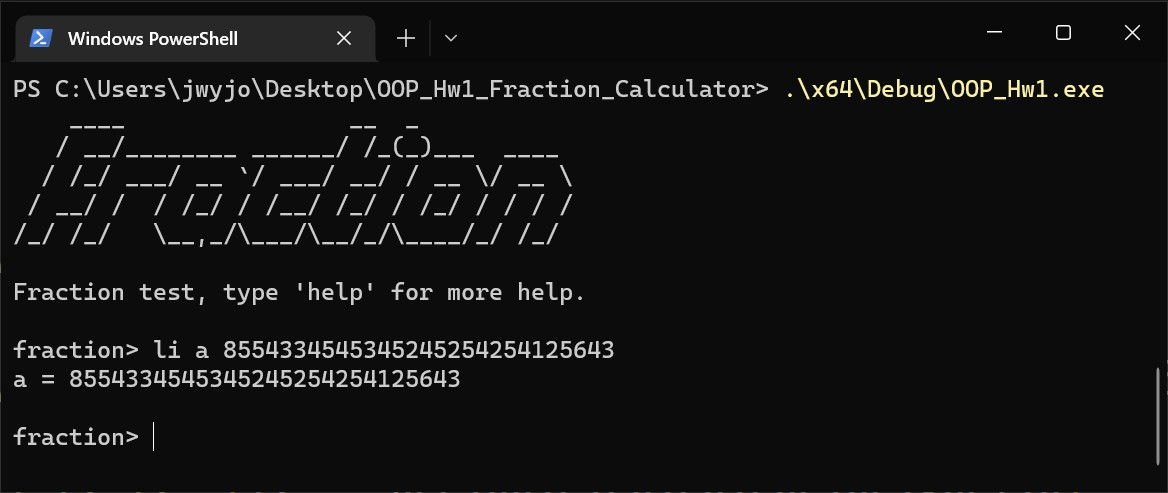
\includegraphics[width=.8\textwidth]{imgs/test_construct_positive_int.jpg}
    \caption{分数的构造-正整数测试结果(符合预期)}
\end{figure}

\paragraph{正分数} 测试用例 \lstinline{li a 85543351/8554334545345245254254125643}
\begin{figure}[H]
    \centering
    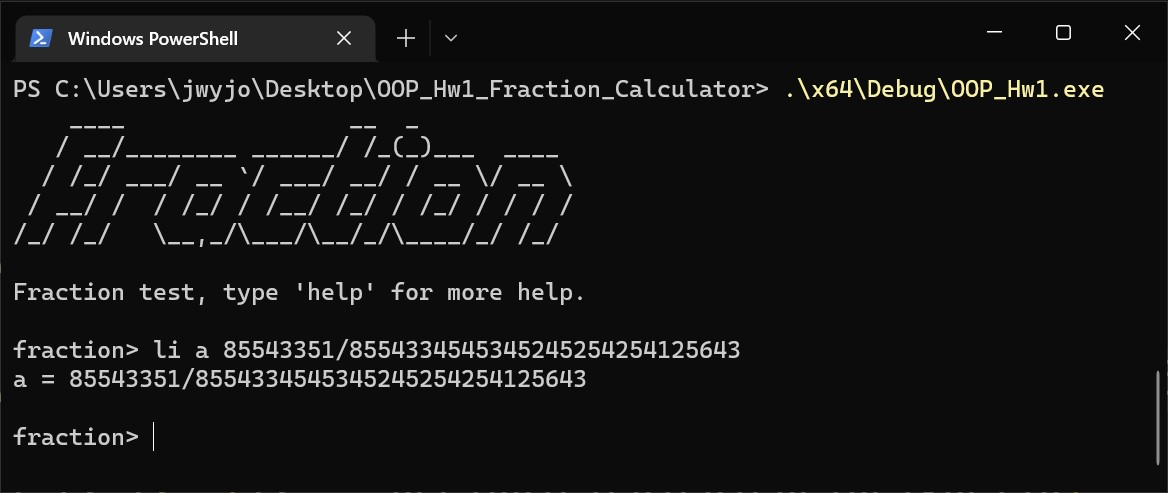
\includegraphics[width=.8\textwidth]{imgs/test_construct_positive_frac.jpg}
    \caption{分数的构造-正分数测试结果(符合预期)}
\end{figure}

\paragraph{负整数} 测试用例 \lstinline{li a -8554334545345245254254125643}
\begin{figure}[H]
    \centering
    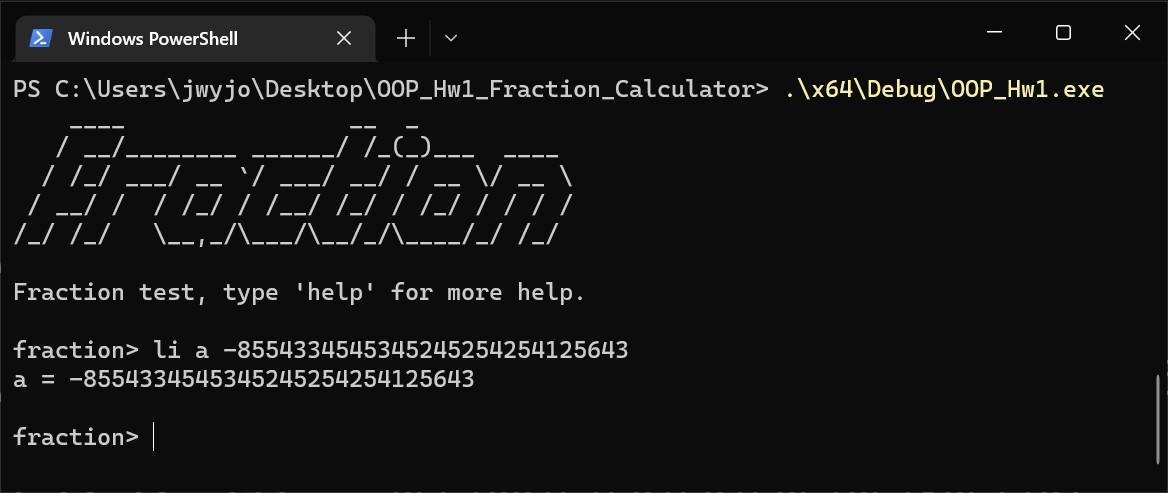
\includegraphics[width=.8\textwidth]{imgs/test_construct_negative_int.jpg}
    \caption{分数的构造-负整数测试结果(符合预期)}
\end{figure}

\paragraph{负分数} 测试用例 \lstinline{li a -85543351/8554334545345245254254125643}
\begin{figure}[H]
    \centering
    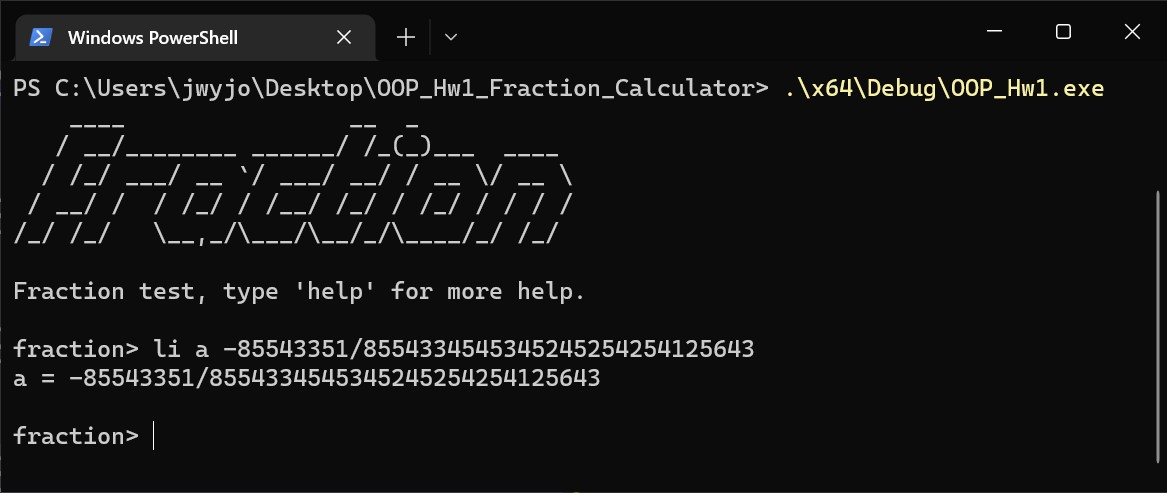
\includegraphics[width=.8\textwidth]{imgs/test_construct_negative_frac.jpg}
    \caption{分数的构造-负分数测试结果(符合预期)}
\end{figure}

\paragraph{零} 测试用例 \lstinline{li a 0}
\begin{figure}[H]
    \centering
    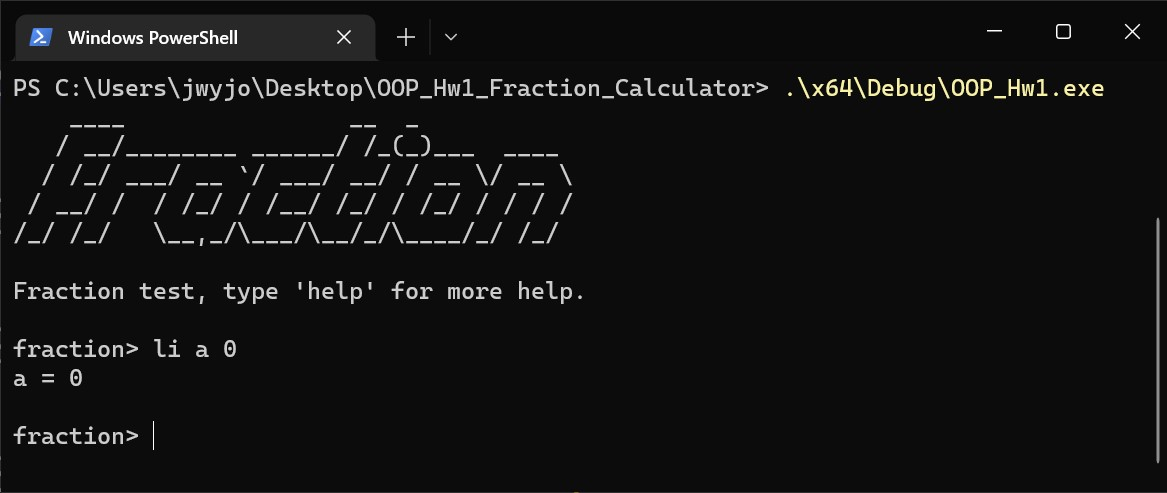
\includegraphics[width=.8\textwidth]{imgs/test_construct_zero.jpg}
    \caption{分数的构造-零的测试结果(符合预期)}
\end{figure}
\paragraph{正浮点数} 测试用例 \lstinline{lf a 0.85543345}
\begin{figure}[H]
    \centering
    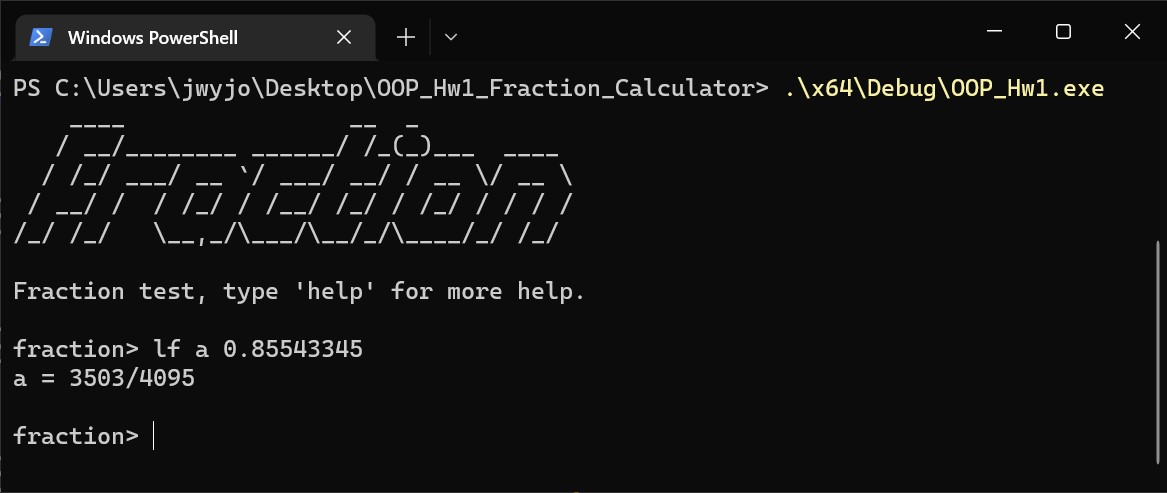
\includegraphics[width=.8\textwidth]{imgs/test_construct_positive_float.jpg}
    \caption{分数的构造-正浮点数测试结果(符合预期)}
\end{figure}

\paragraph{负浮点数} 测试用例 \lstinline{lf a -0.85543345}
\begin{figure}[H]
    \centering
    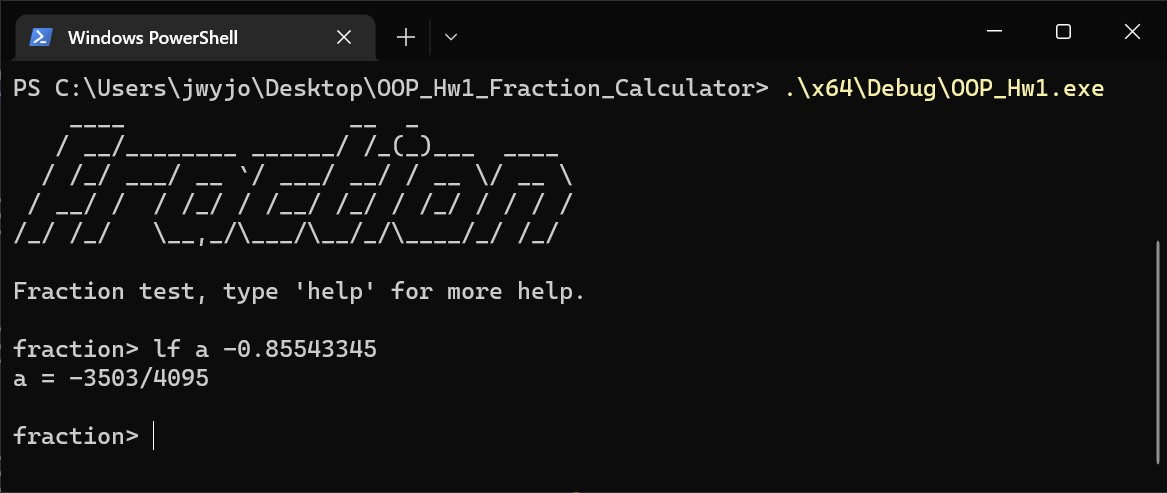
\includegraphics[width=.8\textwidth]{imgs/test_construct_negative_float.jpg}
    \caption{分数的构造-负浮点数测试结果(符合预期)}
\end{figure}

\subsection{分数的化简}

\paragraph{正分数} 测试用例 \lstinline{549755813888/1099511627776}
\begin{figure}[H]
    \centering
    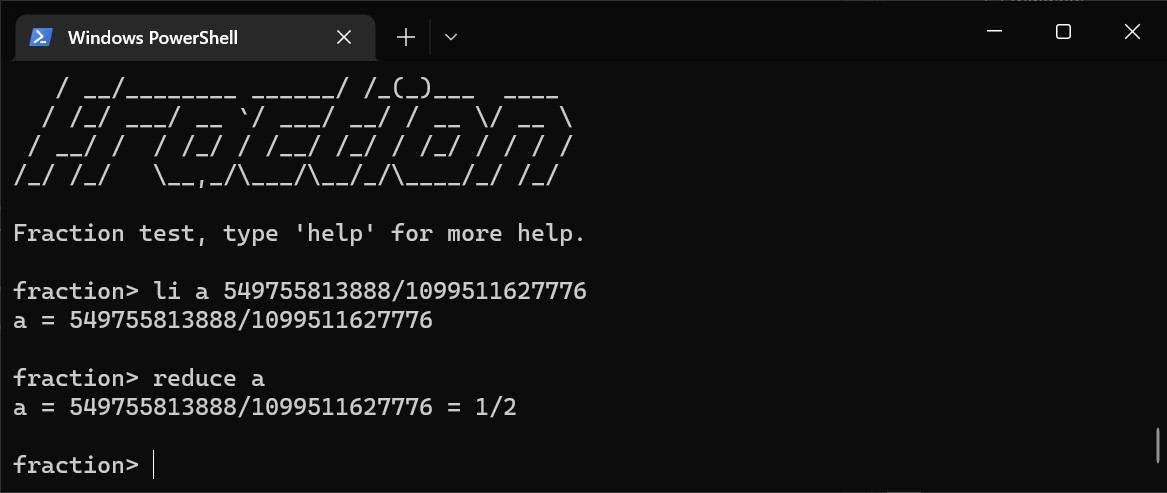
\includegraphics[width=.8\textwidth]{imgs/test_reduce_positive_frac.jpg}
    \caption{分数的化简-正分数测试结果(符合预期)}
\end{figure}

\paragraph{负分数} 测试用例 \lstinline{-549755813888/1099511627776}
\begin{figure}[H]
    \centering
    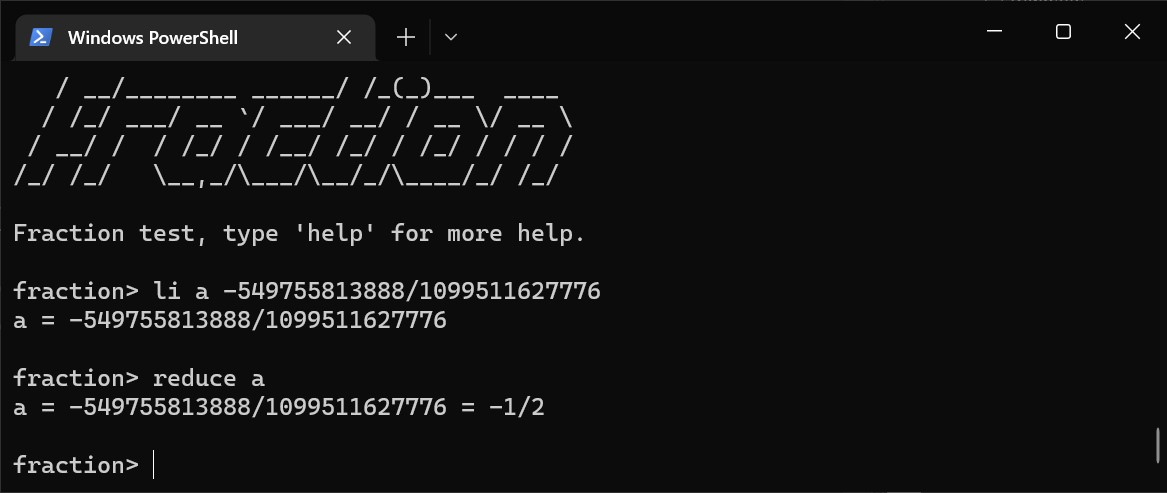
\includegraphics[width=.8\textwidth]{imgs/test_reduce_negative_frac.jpg}
    \caption{分数的化简-负分数测试结果(符合预期)}
\end{figure}

\paragraph{正整数} 测试用例 \lstinline{1099511627776/549755813888}
\begin{figure}[H]
    \centering
    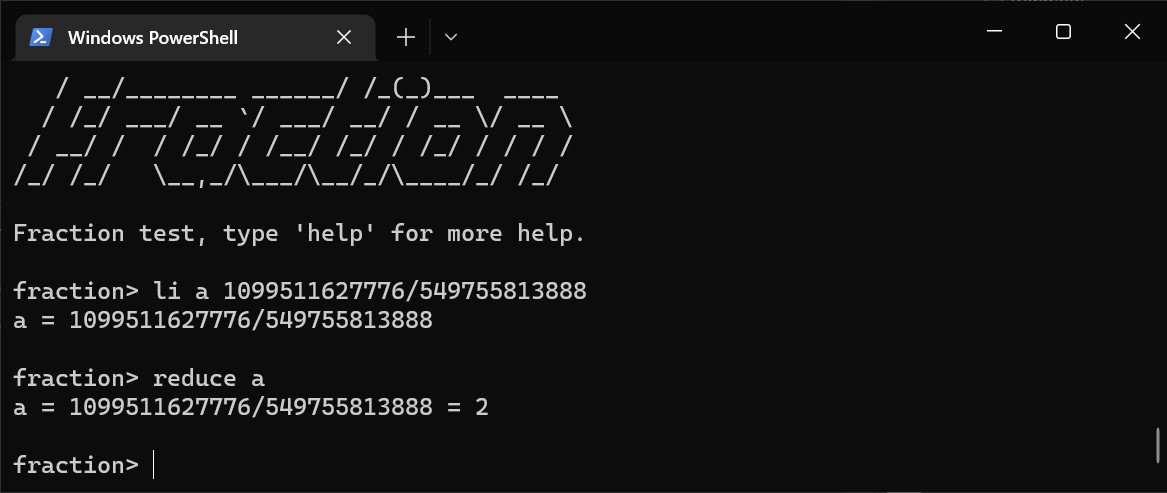
\includegraphics[width=.8\textwidth]{imgs/test_reduce_positive_int.jpg}
    \caption{分数的化简-正整数测试结果(符合预期)}
\end{figure}

\paragraph{负整数} 测试用例 \lstinline{-1099511627776/549755813888}
\begin{figure}[H]
    \centering
    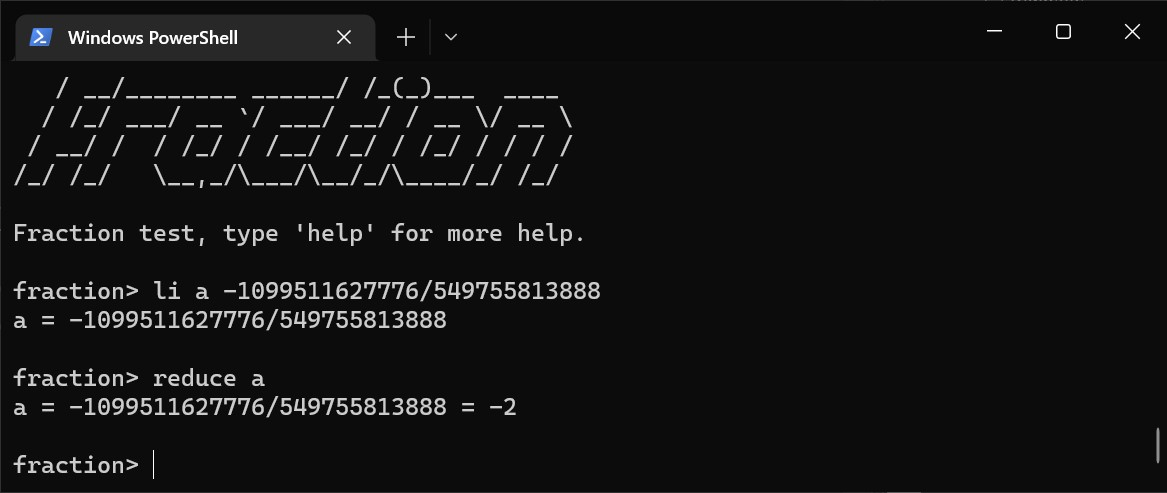
\includegraphics[width=.8\textwidth]{imgs/test_reduce_negative_int.jpg}
    \caption{分数的化简-负整数测试结果(符合预期)}
\end{figure}

\paragraph{零分母} 测试用例 \lstinline{1/0}
\begin{figure}[H]
    \centering
    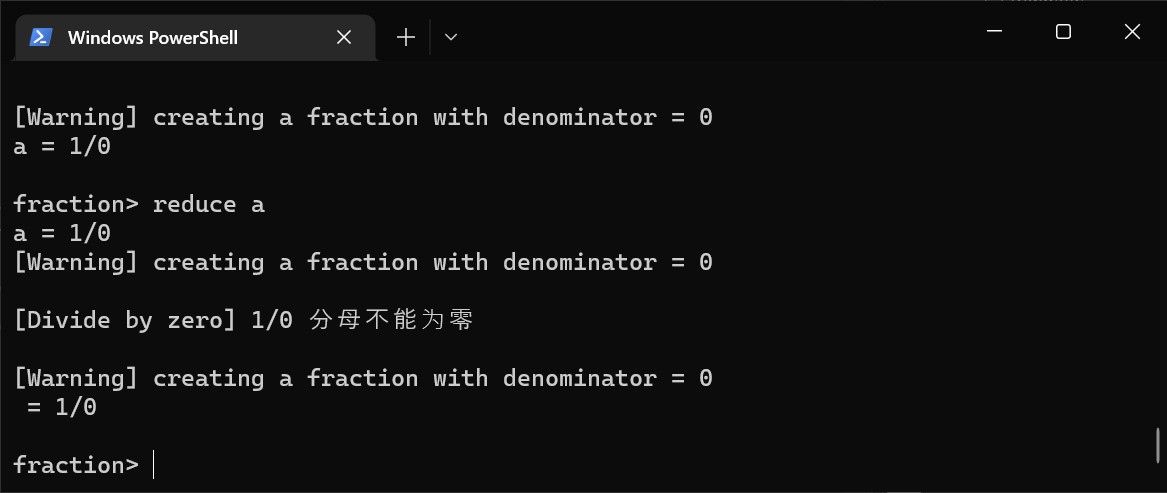
\includegraphics[width=.8\textwidth]{imgs/test_reduce_zero1.jpg}
    \caption{分数的化简-零分母测试结果(符合预期)}
\end{figure}

\paragraph{零分子} 测试用例 \lstinline{0/1099511627776}
\begin{figure}[H]
    \centering
    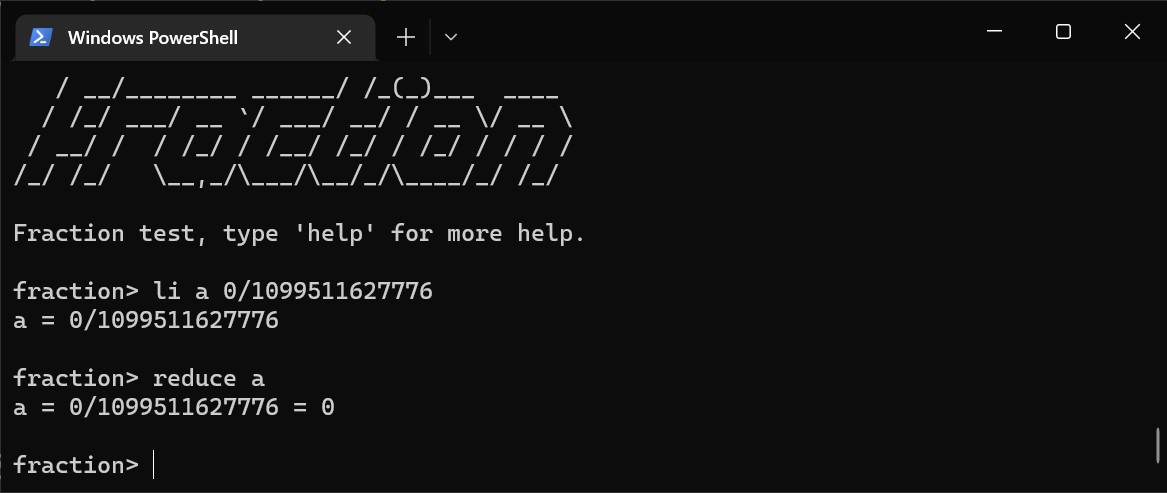
\includegraphics[width=.8\textwidth]{imgs/test_reduce_zero2.jpg}
    \caption{分数的化简-零分母测试结果(符合预期)}
\end{figure}

\subsection{取负数}

\paragraph{正数} 测试用例 \lstinline{549755813888/1099511627776}
\begin{figure}[H]
    \centering
    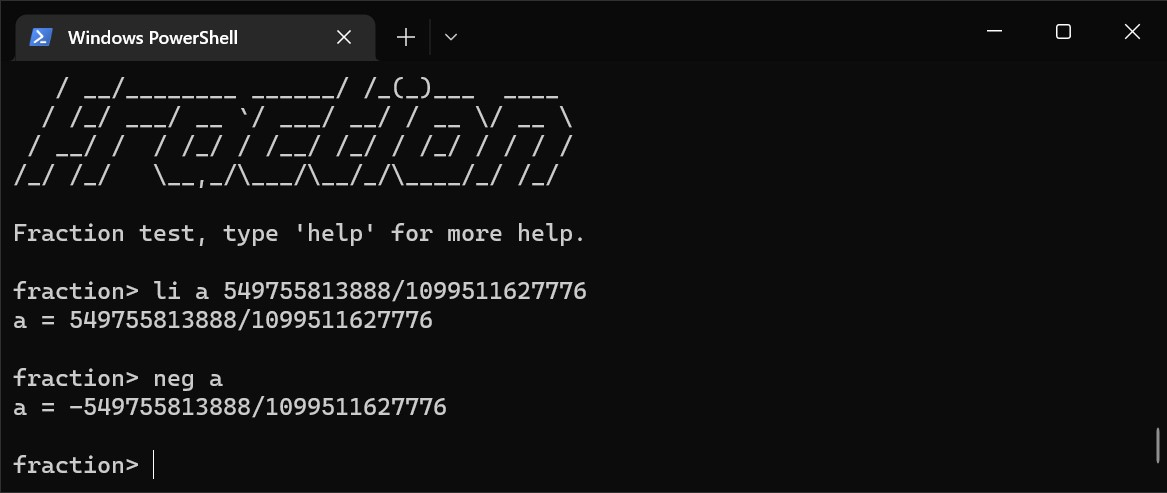
\includegraphics[width=.8\textwidth]{imgs/test_neg_positive_frac.jpg}
    \caption{取负数-正分数测试结果(符合预期)}
\end{figure}

\paragraph{负数} 测试用例 \lstinline{-549755813888/1099511627776}
\begin{figure}[H]
    \centering
    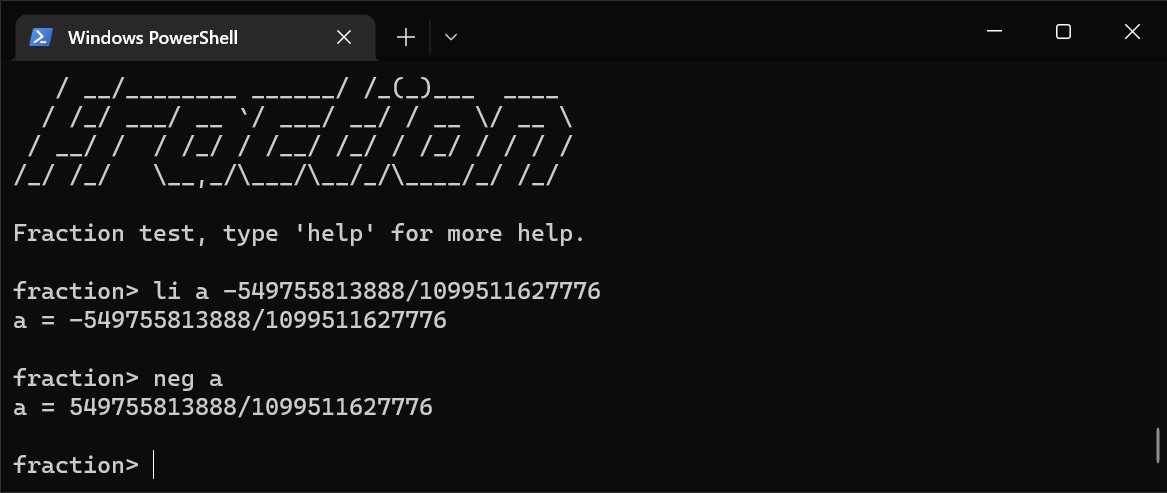
\includegraphics[width=.8\textwidth]{imgs/test_neg_negative_frac.jpg}
    \caption{取负数-负分数测试结果(符合预期)}
\end{figure}

\paragraph{零分母} 测试用例 \lstinline{1/0}
\begin{figure}[H]
    \centering
    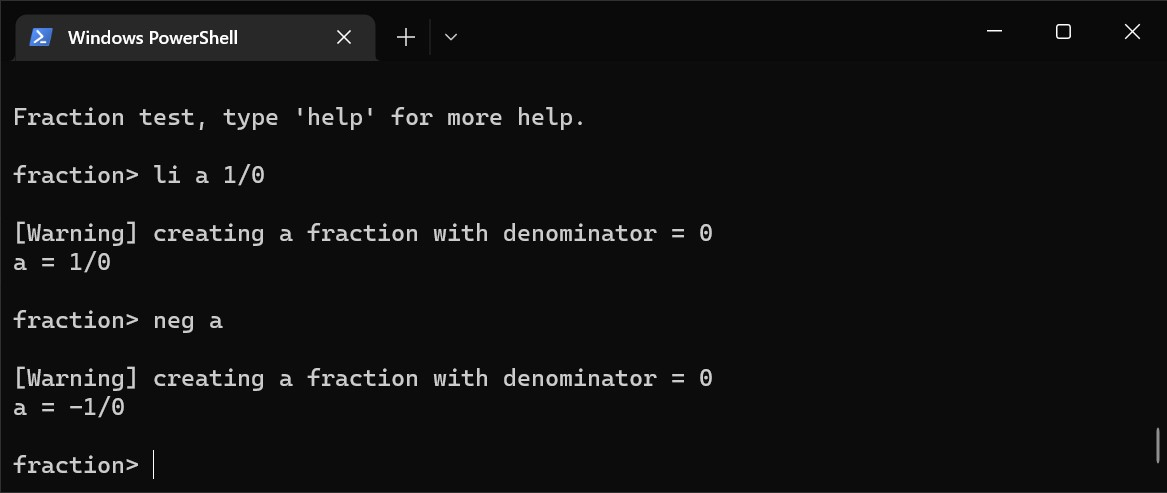
\includegraphics[width=.8\textwidth]{imgs/test_neg_zero1.jpg}
    \caption{取负数-零分母测试结果(符合预期)}
\end{figure}

\paragraph{零分子} 测试用例 \lstinline{0/1099511627776}
\begin{figure}[H]
    \centering
    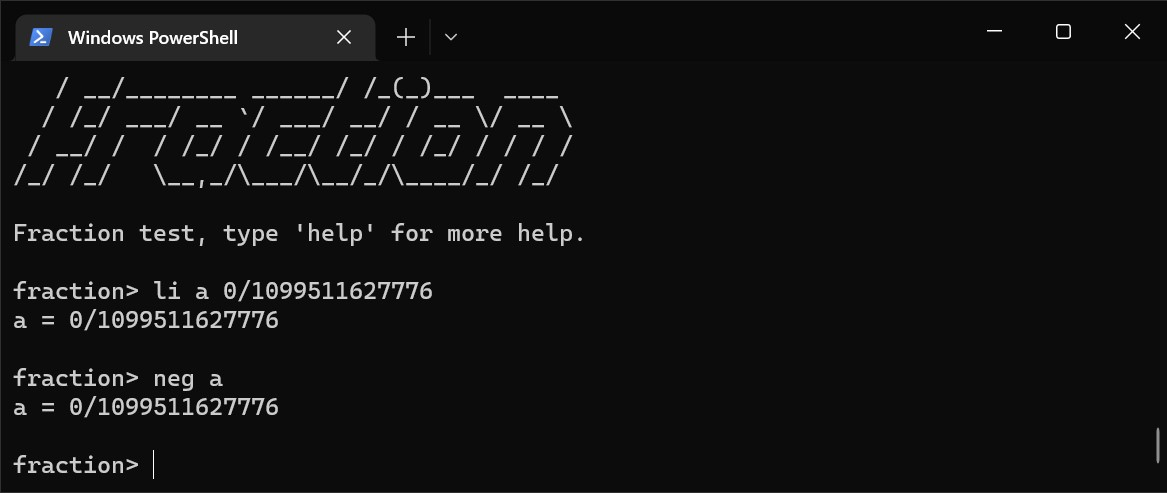
\includegraphics[width=.8\textwidth]{imgs/test_neg_zero2.jpg}
    \caption{取负数-零分母测试结果(符合预期)}
\end{figure}

\subsection{取倒数}

\paragraph{正数} 测试用例 \lstinline{549755813888/1099511627776}
\begin{figure}[H]
    \centering
    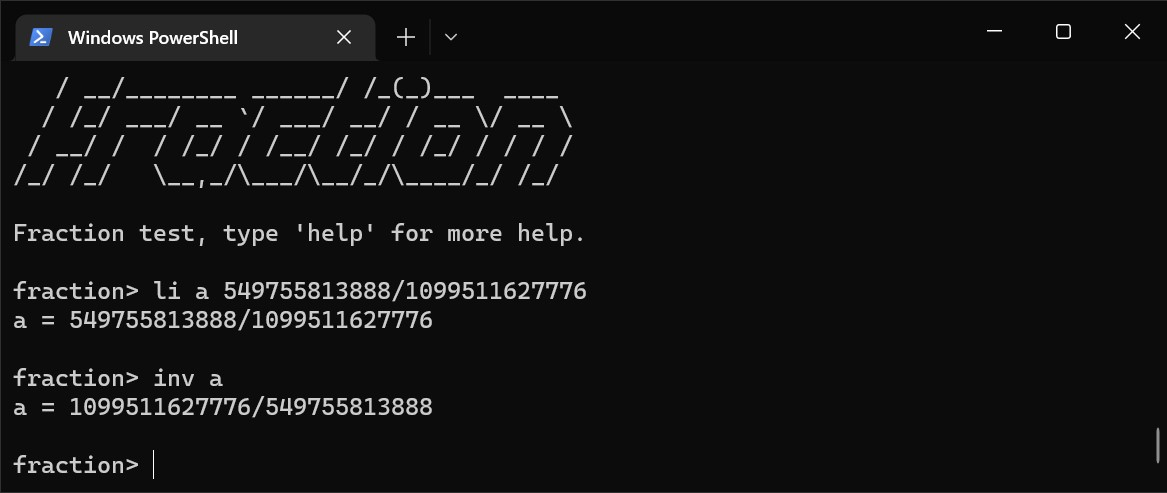
\includegraphics[width=.8\textwidth]{imgs/test_inv_positive_frac.jpg}
    \caption{取倒数-正分数测试结果(符合预期)}
\end{figure}

\paragraph{负数} 测试用例 \lstinline{-549755813888/1099511627776}
\begin{figure}[H]
    \centering
    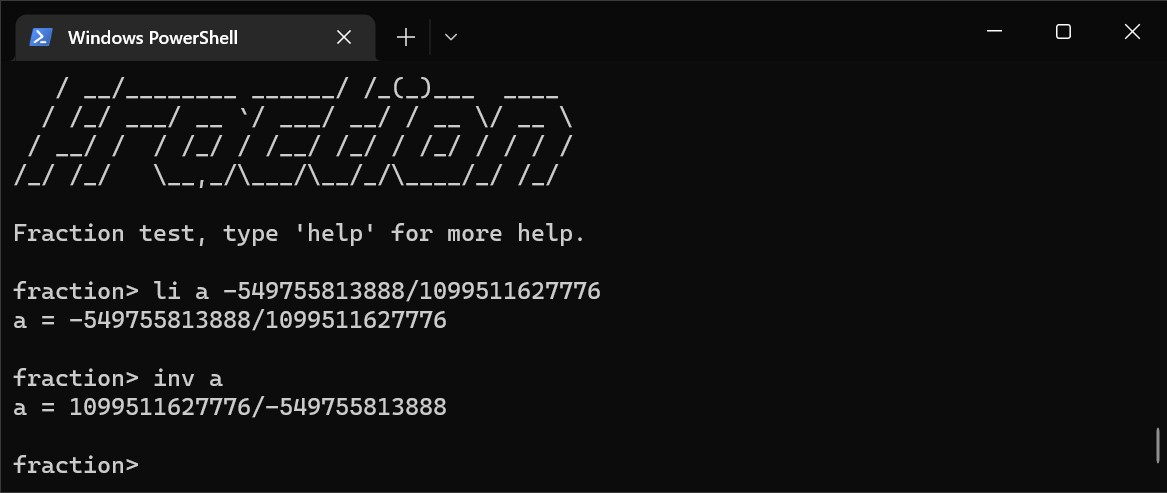
\includegraphics[width=.8\textwidth]{imgs/test_inv_negative_frac.jpg}
    \caption{取倒数-负分数测试结果(符合预期)}
\end{figure}

\paragraph{零分母} 测试用例 \lstinline{1/0}
\begin{figure}[H]
    \centering
    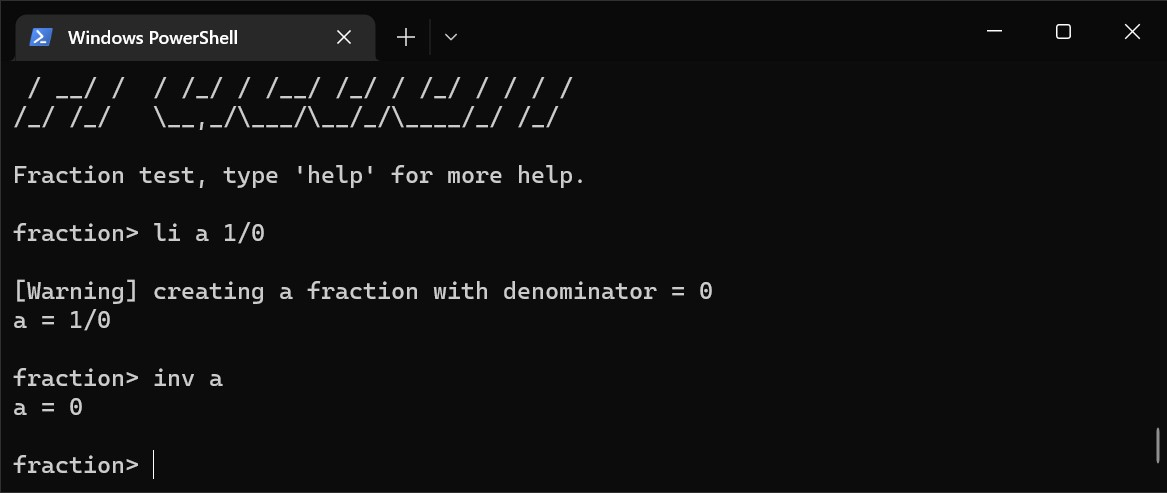
\includegraphics[width=.8\textwidth]{imgs/test_inv_zero1.jpg}
    \caption{取倒数-零分母测试结果(符合预期)}
\end{figure}

\paragraph{零分子} 测试用例 \lstinline{0/1099511627776}
\begin{figure}[H]
    \centering
    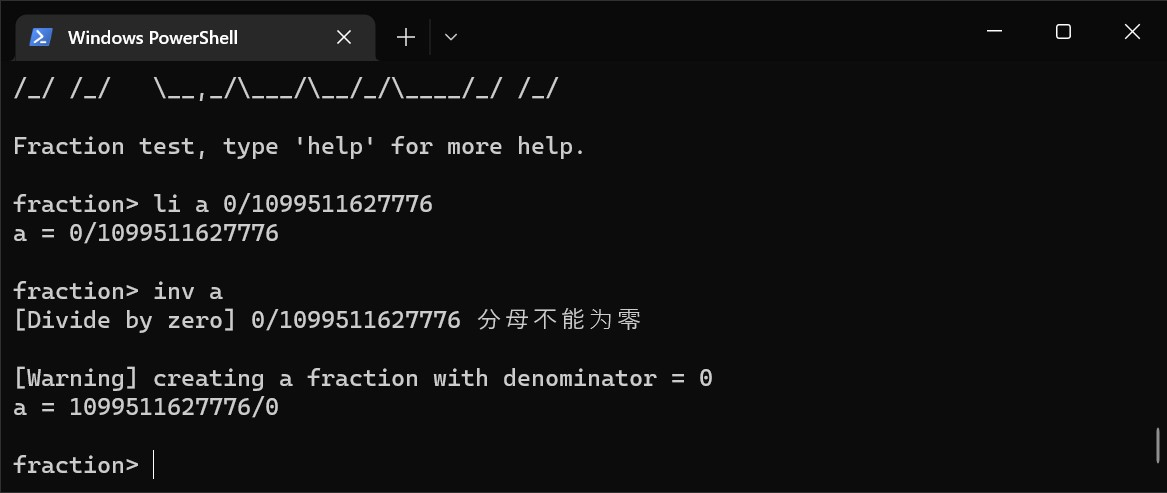
\includegraphics[width=.8\textwidth]{imgs/test_inv_zero2.jpg}
    \caption{取倒数-零分母测试结果(符合预期)}
\end{figure}

\subsection{四则运算}

\subsection{比较运算}

\section{设计思路}

\subsection{分层开发}

\subsection{组合优于继承}

\subsection{类图}

\section{实现细节}

\subsection{高精度正整数类}

\subsection{高精度整数类}

\subsection{高精度分数类}

\section{作业小结}

\end{document}